\documentclass[11pt,a4paper]{article}
\usepackage[margin=2.3cm]{geometry}
\usepackage{graphicx,booktabs,amsmath,amssymb,hyperref,caption,subcaption,array}
\usepackage[T1]{fontenc}\usepackage{lmodern}
\hypersetup{colorlinks=true,linkcolor=black,urlcolor=blue}
\emergencystretch=3em\setlength{\parskip}{0.5em}\setlength{\parindent}{0pt}
\title{Index Selection on PostgreSQL: Reproducing the Kossmann et al.\ Evaluation and Adding Budget-Aware Tuning (Wii, Esc)}
\author{Arijit Mandal \and Rameez Wahid\\ CS 631 Databases, IIT Bombay}
\date{25 November 2026}
\begin{document}
\maketitle

\begin{abstract}
We reproduce the TPC-H (scale factor 10) experiment of Kossmann et al.\ (PVLDB 13(11), 2020) on PostgreSQL 18.7 with the authors' platform, and extend it with budget-aware index tuning: a two-phase greedy tuner with the call-skipping mechanism Wii (Wang et al., SIGMOD 2024) and the early-stopping checker Esc (Wang et al., PVLDB 2025), both implemented by us from the papers because no code was available. The original study's picture is reproduced in shape: the same cost cliff, a cluster of near-equal algorithms, and the same ordering of run times; the cliff sits at a smaller budget, CoPhy ends about 4 points better, and run times are 2--10$\times$ lower. Judged by the optimizer's estimates, Wii finds indexes with 96\% of the improvement of the unrestricted tuner using 14\% of its what-if calls (32.7\% against 33.9\% improvement, 430 against 3\,040 calls; four statistics draws), and against the original eight algorithms at 10\,GB the tuner with Wii reaches 68.3\% relative cost with 430 calls, where CoPhy reaches 66.3\% with 23\,066. Esc saves 5--28\% of the calls in the storage-limited setting, with a storage-aware bound that we added (on synthetic data Esc never stopped without it; we did not measure its effect on TPC-H), and it adds nothing on top of Wii. These results rest on estimates. When we built the indexes chosen at a 5\,GB budget and ran the queries, only the plain two-phase greedy was faster than no indexes (by 35\%); Extend, Relaxation, Wii, Esc and Wii~+~Esc were 3--40\% slower, although all six were estimated to improve the workload by 26--29\%. The estimated quality of an algorithm therefore does not show how good its indexes are in practice, and this limits every comparison in the report.
\end{abstract}

\section{Introduction}
Index selection algorithms choose indexes for a workload under a storage or count budget, usually by asking the optimizer for the cost of the workload under hypothetical (what-if) indexes. Kossmann et al.\ compared eight algorithms (Extend, Relaxation, DTA, CoPhy, DB2Advis, AutoAdmin, Drop, Dexter) on several workloads and DBMSs. The project had three objectives:
\begin{enumerate}
\item \textbf{Reproduce} the TPC-H SF10 evaluation on a current PostgreSQL (Section~\ref{sec:repro}).
\item \textbf{Extend} it with budget-aware tuning, Wii and Esc, and compare them with the original eight (Sections~\ref{sec:setup}--\ref{sec:compare}).
\item \textbf{Execute} the selected indexes and time the queries, instead of relying on estimates (Section~\ref{sec:exec}).
\end{enumerate}
\textbf{Contributions.} A reproduction with three repetitions per point; an implementation of a budget-aware two-phase greedy with Wii, Esc-B and their evaluation; three additions of our own to Esc (the storage budget in the simulated greedy, a storage-aware upper bound, and an optional clamp that is a heuristic); and a real-execution check that shows the limits of estimate-based comparisons. What is \emph{not} done is listed in Section~\ref{sec:limits}.

\section{Reproduction of the original evaluation}\label{sec:repro}
\textbf{Setup.} TPC-H SF10, 19 queries (2, 17 and 20 excluded, as in the paper). The metric is the relative workload cost: the optimizer's estimate for the workload with the selected hypothetical indexes divided by the estimate without indexes. All eight algorithms ran with the repository configuration \texttt{tpch\_sf10\_paper.json}: storage-budget algorithms at 16 budgets from 250 to 15\,000\,MB, AutoAdmin and Drop at 1--13 indexes, Dexter at 5 thresholds; every point three times (112 parameter points). Differences from the paper: PostgreSQL 18.7 instead of 12.1, HypoPG 1.4.5, Dexter 0.6.3, CoPhy solved with Gurobi 13 through PuLP 3 and index width 3 in the main run (the paper states 2), and different hardware.

\begin{figure}[h]\centering
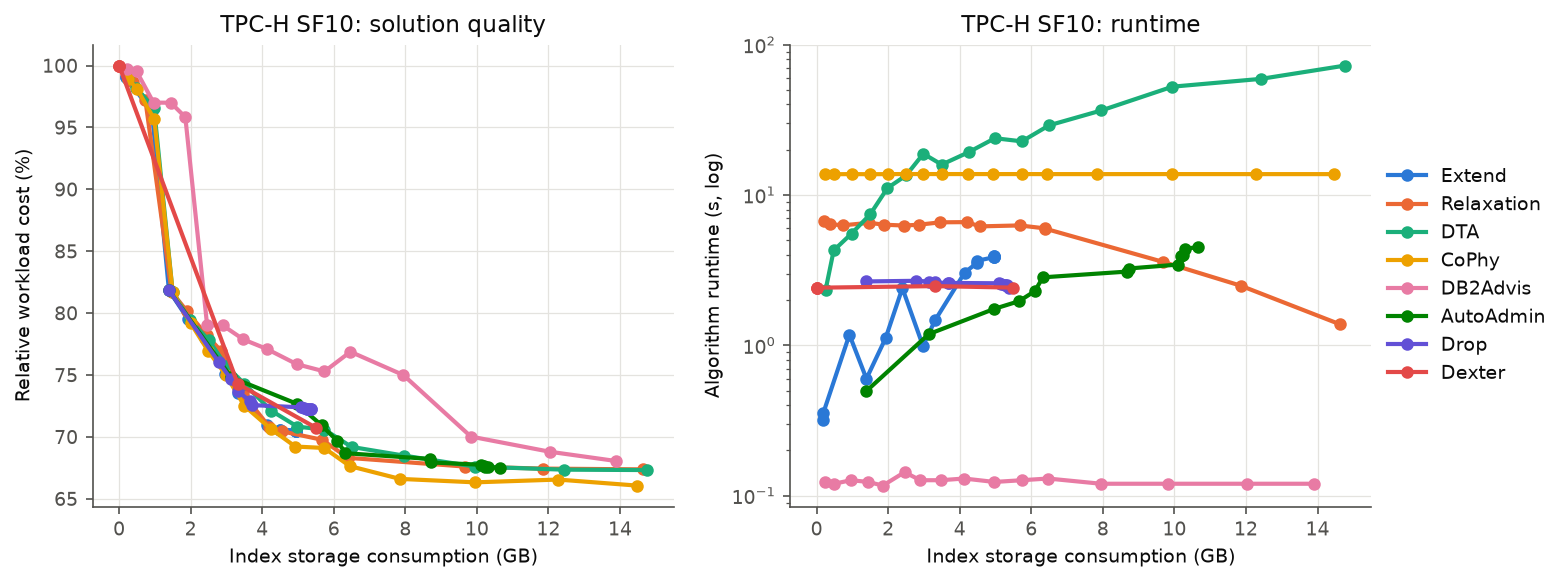
\includegraphics[width=\textwidth]{tpch_sf10_reproduction.png}
\caption{TPC-H SF10: relative workload cost (left) and algorithm run time (right, log scale), means of three repetitions.}\label{fig:repro}
\end{figure}

\textbf{What reproduces.} All storage-budget algorithms except DB2Advis follow almost the same curve. Nothing helps below about 1.4\,GB; once the budget admits one large index on \texttt{lineitem.l\_orderkey}, the cost drops from about 96\% to 82\% for every algorithm. Beyond 6\,GB, Relaxation, DTA, AutoAdmin and CoPhy end within 67.3--67.7\% (CoPhy re-run at width 2), Extend at 70.5\%. DB2Advis is fast (0.1\,s) but needs more space for the same quality. The ordering of run times (DB2Advis $\ll$ Extend, Drop, Dexter $<$ Relaxation $<$ CoPhy, DTA growing with the budget) agrees with the paper, and so does Dexter's operating point (70.7\% at about 5.4\,GB).

\textbf{What differs.} (1) The cliff is at about 1.4\,GB instead of the paper's 2\,GB; HypoPG's size estimate for the large index is clearly smaller, and we did not isolate the cause (PostgreSQL version and the newer estimator are candidates). (2) CoPhy is among the best here, but not in the paper. Re-running it at width 2 removes only about 1 point; about 4 points remain unexplained. (3) Absolute run times are 2--10$\times$ lower with the same shapes; we attribute this to newer hardware and software without having tested it, and we compare orderings, not seconds. Paper values were read off its figures (accuracy about $\pm$1--2 points).

\textbf{Variability.} \texttt{ANALYZE} samples rows randomly, so each repetition sees different statistics. The largest spread over repetitions is 3.15 points for DTA, 2.51 for CoPhy, 1.70 for Relaxation, 1.57 for DB2Advis, 1.09 for AutoAdmin, 1.07 for Extend, 0.39 for Drop and 0.29 for Dexter. Differences of one to two points between Relaxation, DTA, AutoAdmin and CoPhy at large budgets are within noise, and we do not rank them.

